\section{Mechanics of a System of Particles}

In generalizing the ideas of the previous section to systems of many particles, we must distinguish between the \emph{external forces} acting on the particles due to sources outside the system, and \emph{internal forces} on, say, some particle \(i\) due to all other particles in the system. Thus, the equation of motion (Newton's second law) for the \(i\)th particle is written as
\begin{equation}
    \sum_j\symbf{F}_{ji}+\symbf{F}_i^{\left(e\right)}=\dot{\symbf{p}}_i,\label{eq:1.19}
\end{equation}
where \(\symbf{F}_i^{\left(e\right)}\) stands for an external force, and \(\symbf{F}_{ji}\) is the internal force on the \(i\)th particle due to the \(j\)th particle (\(\symbf{F}_{ii}\) naturally, is zero). We shall assume that the \(\symbf{F}_{ij}\) (like the \(\symbf{F}_i^{\left(e\right)}\)) obey Newton's third law of motion in its original form: that the forces two particles exert on each other are equal and opposite. This assumption (which does not hold for all types of forces) is sometimes referred to as the \emph{weak law of action and reaction}.

Summed over all particles, Eq.~\eqref{eq:1.19} takes the form
\begin{equation}
    \odv*[2]{\sum_im_i\symbf{r}_i}{t}=\sum_i\symbf{F}_i^{\left(e\right)}+\sum_{\substack{i,j\\i\ne j}}\symbf{F}_{ji}.\label{eq:1.20}
\end{equation}
The first sum on the right is simply the total external force \(\symbf{F}^{\left(e\right)}\), while the second term vanishes, since the law of action and reaction states that each pair \(\symbf{F}_{ij}+\symbf{F}_{ji}\) is zero. To reduce the left-hand side, we define a vector \(\symbf{R}\) as the average of the radius vectors of the particles, weighted in proportion to their mass:
\begin{equation}
    \symbf{R}=\frac{\sum m_i\symbf{r}_i}{\sum m_i}=\frac{\sum m_i\symbf{r}_i}{M}.\label{eq:1.21}
\end{equation}
The vector \(\symbf{R}\) defines a point known as the \emph{center of mass}, or more loosely as the center of gravity, of the system (cf. Fig.~\ref{fig:1.1}). With this definition, \eqref{eq:1.20} reduces to
\begin{equation}
    M\odv[2]{\symbf{R}}{t}=\sum_i\symbf{F}_i^{\left(e\right)}\equiv\symbf{F}^{\left(e\right)},\label{eq:1.22}
\end{equation}
which states that the center of mass moves as if the total external force were acting on the entire mass of the system concentrated at the center of mass. Purely internal forces, if they obey Newton's third law, therefore have no effect on the motion of the center of mass. An oft-quoted example is the motion of an exploding shell---the center of mass of the fragments traveling as if the shell were still in a single piece (neglecting air resistance). The same principle is involved in jet and rocket propulsion. In order that the motion of the center of mass be unaffected, the ejection of the exhaust gases at high velocity must be counterbalanced by the forward motion of the vehicle at a slower velocity.

\begin{figure}[htbp]
    \centering
    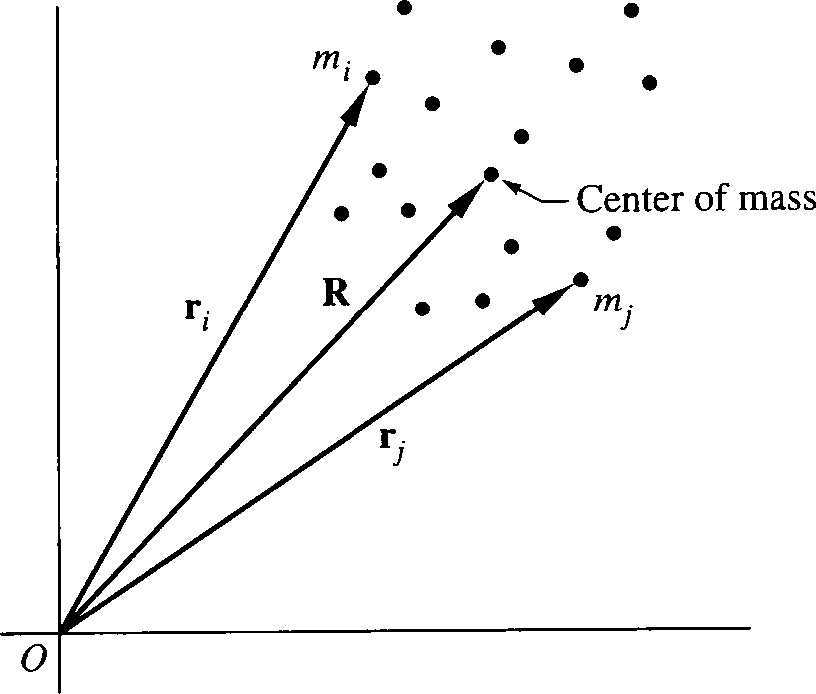
\includegraphics[scale = 0.225]{01/figures/1.1}
    \caption{The center of mass of a system of particles.}
    \label{fig:1.1}
\end{figure}

By Eq.~\eqref{eq:1.21} the total linear momentum of the system,
\begin{equation}
    \symbf{P}=\sum m_i\odv{\symbf{r}_i}{t}=M\odv{\symbf{R}}{t},\label{eq:1.23}
\end{equation}
is the total mass of the system times the velocity of the center of mass. Consequently, the equation of motion for the center of mass, \eqref{eq:1.23}, can be restated as the
\begin{theorem}[Conservation Theorem for the Linear Momentum of a System of Particles]
    If the total external force is zero, the total linear momentum is conserved.
\end{theorem}

We obtain the total angular momentum of the system by forming the cross product \(\symbf{r}_i\vectimes\symbf{p}_i\) and summing over \(i\). If this operation is performed in Eq.~\eqref{eq:1.19}, there results, with the aid of the identity, Eq.~\eqref{eq:1.10},
\begin{equation}
    \sum_i\left(\symbf{r}_i\vectimes\dot{\symbf{p}}_i\right)=\sum_i\odv*{\left(\symbf{r}_i\vectimes\symbf{p}_i\right)}{t}=\dot{\symbf{L}}=\sum_i\symbf{r}_i\vectimes\symbf{F}_i^{\left(e\right)}+\sum_{\substack{i,j\\i\ne j}}\symbf{r}_i\vectimes\symbf{F}_{ji}.\label{eq:1.24}
\end{equation}
The last term on the right in \eqref{eq:1.24} can be considered a sum of the pairs of the form
\begin{equation}
    \symbf{r}_i\vectimes\symbf{F}_{ji}+\symbf{r}_j\vectimes\symbf{F}_{ij}=\left(\symbf{r}_i-\symbf{r}_j\right)\vectimes\symbf{F}_{ji},\label{eq:1.25}
\end{equation}
using the equality of action and reaction. But \(\symbf{r}_i-\symbf{r}_j\) is identical with the vector \(\symbf{r}_{ij}\) from \(j\) to \(i\) (cf. Fig.~\ref{fig:1.2}), so that the right-hand side of Eq.~\eqref{eq:1.25} can be written as
\begin{equation*}
    \symbf{r}_{ij}\vectimes\symbf{F}_{ji}.
\end{equation*}
If the internal forces between two particles, in addition to being equal and opposite, also lie along the line joining the particles---a condition known as the \emph{strong law of action and reaction}---then all of these cross products vanish. The sum over pairs is zero under this assumption and Eq.~\eqref{eq:1.24} may be written in the form
\begin{equation}
    \odv{\symbf{L}}{t}=\symbf{N}^{\left(e\right)}.\label{eq:1.26}
\end{equation}
The time derivative of the total angular momentum is thus equal to the moment of the external force about the given point. Corresponding to Eq.~\eqref{eq:1.26} is the
\begin{theorem}[Conservation Theorem for Total Angular Momentum]
    \(\symbf{L}\) is constant in time if the applied (external) torque is zero.
\end{theorem}

\begin{figure}[htbp]
    \centering
    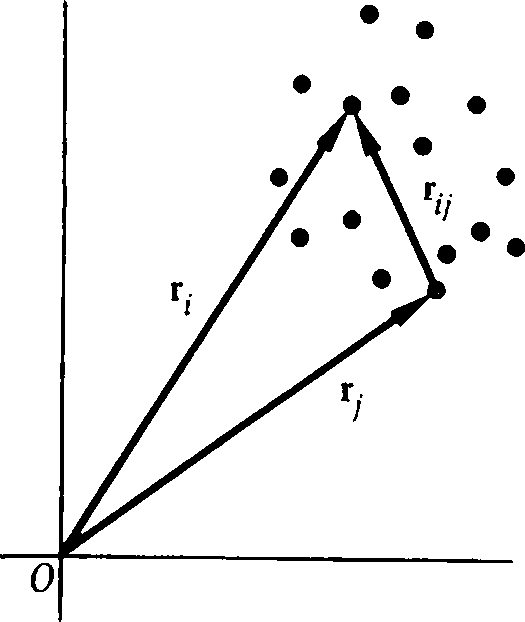
\includegraphics[scale = 0.225]{01/figures/1.2}
    \caption{The vector \(\symbf{r}_{ij}\) between the \(i\)th and \(j\)th particles.}
    \label{fig:1.2}
\end{figure}

(It is perhaps worthwhile to emphasize that this is a \emph{vector} theorem; i.e., \(L_z\) will be conserved if \(N_z^{\left(e\right)}\) is zero, even if \(N_x^{\left(e\right)}\) and \(N_y^{\left(e\right)}\) are not zero.)

Note that the conservation of linear momentum in the absence of applied forces assumes that the weak law of action and reaction is valid for the internal forces. The conservation of the total angular momentum of the system in the absence of applied torques requires the validity of the strong law of action and reaction—that the internal forces in addition be \emph{central}. Many of the familiar physical forces, such as that of gravity, satisfy the strong form of the law. But it is possible to find forces for which action and reaction are equal even though the forces are not central (see below). In a system involving moving charges, the forces between the charges predicted by the Biot-Savart law may indeed violate both forms of the action and reaction law.\footnote{If two charges are moving uniformly with parallel velocity vectors that are not perpendicular to the line joining the charges, then the net mutual forces are equal and opposite but do not lie along the vector between the charges. Consider, further, two charges moving (instantaneously) so as to ``cross the T," i.e., one charge moving directly at the other, which in turn is moving at right angles to the first. Then the second charge exerts a nonvanishing magnetic force on the first, without experiencing any magnetic reaction force at that instant.} Equations~\eqref{eq:1.23} and \eqref{eq:1.26}, and their corresponding conservation theorems, are not applicable in such cases, at least in the form given here. Usually it is then possible to find some generalization of \(\symbf{P}\) or \(\symbf{L}\) that is conserved. Thus, in an isolated system of moving charges it is the sum of the mechanical angular momentum and the electromagnetic ``angular momentum" of the field that is conserved.

Equation~\eqref{eq:1.23} states that the total linear momentum of the system 1s the same as if the entire mass were concentrated at the center of mass and moving with it. The analogous theorem for angular momentum is more complicated. With the origin \(O\) as reference point, the total angular momentum of the system is
\begin{equation*}
    \symbf{L}=\sum_i\symbf{r}_i\vectimes\symbf{p}_i.
\end{equation*}
Let \(\symbf{R}\) be the radius vector from \(O\) to the center of mass, and let \(\symbf{r}_i'\) be the radius vector from the center of mass to the \(i\)th particle. Then we have (cf. Fig.~\ref{fig:1.3})
\begin{equation}
    \symbf{r}_i=\symbf{r}_i'+\symbf{R}\label{eq:1.27}
\end{equation}
and
\begin{equation*}
    \symbf{v}_i=\symbf{v}_i'+\symbf{v}
\end{equation*}
where
\begin{equation*}
    \symbf{v}=\odv{\symbf{R}}{t}
\end{equation*}
is the velocity of the center of mass relative to \(O\), and
\begin{equation*}
    \symbf{v}_i'=\odv{\symbf{r}_i'}{t}
\end{equation*}
is the velocity of the \(i\)th particle relative to the center of mass of the system. Using Eq.~\eqref{eq:1.27}, the total angular momentum takes on the form
\begin{equation*}
    \symbf{L}=\sum_i\symbf{R}\vectimes m_i\symbf{v}+\sum_i\symbf{r}_i'\vectimes m_i\symbf{v}_i'+\left(\sum_im_i\symbf{r}_i'\right)\vectimes\symbf{v}+\symbf{R}\vectimes\odv*{\sum_im_i\symbf{r}_i'}{t}.
\end{equation*}
The last two terms in this expression vanish, for both contain the factor \(\sum m_i\symbf{r}_i'\), which, it will be recognized, defines the radius vector of the center of mass in the very coordinate system whose origin is the center of mass and is therefore a null vector. Rewriting the remaining terms, the total angular momentum about \(O\) is
\begin{equation}
    \symbf{L}=\symbf{R}\vectimes M\symbf{v}+\sum_i\symbf{r}_i'\vectimes\symbf{p}_i'.\label{eq:1.28}
\end{equation}
In words, Eq.~\eqref{eq:1.28} says that the total angular momentum about a point \(O\) is the angular momentum of motion concentrated at the center of mass, plus the angular momentum of motion about the center of mass. The form of Eq.~\eqref{eq:1.28} emphasizes that in general \(\symbf{L}\) depends on the origin \(O\), through the vector \(\symbf{R}\). Only if the center of mass is at rest with respect to \(O\) will the angular momentum be independent of the point of reference. In this case, the first term in \eqref{eq:1.28} vanishes, and \(\symbf{L}\) always reduces to the angular momentum taken about the center of mass.

\begin{figure}[htbp]
    \centering
    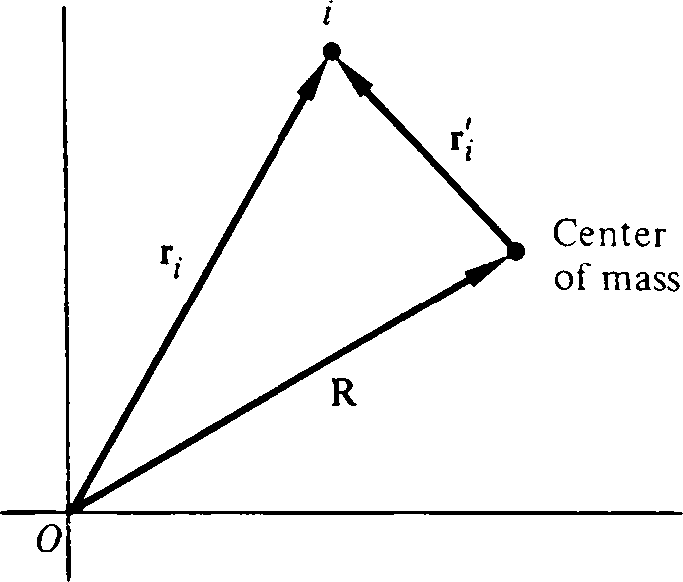
\includegraphics[scale = 0.225]{01/figures/1.3}
    \caption{The vectors involved in the shift of reference point for the angular momentum.}
    \label{fig:1.3}
\end{figure}

Finally, let us consider the energy equation. As in the case of a single particle, we calculate the work done by all forces in moving the system from an initial configuration \(1\), to a final configuration \(2\):
\begin{equation}
    W_{12}=\sum_i\int_1^2\symbf{F}_i\cdot\odif{\symbf{s}_i}=\sum_i\int_1^2\symbf{F}_i^{\left(e\right)}\cdot\odif{\symbf{s}_i}+\sum_{\substack{i,j\\i\ne j}}\int_1^2\symbf{F}_{ji}\cdot\odif{\symbf{s}_i}.\label{eq:1.29}
\end{equation}
Again, the equations of motion can be used to reduce the integrals to
\begin{equation*}
    \sum_i\int_1^2\symbf{F}_i\cdot\odif{\symbf{s}_i}=\sum_i\int_1^2m_i\dot{\symbf{v}}_i\cdot\symbf{v}_i\odif{t}=\sum_i\int_1^2\odif{\left(\frac{1}{2}m_iv_i^2\right)}.
\end{equation*}
Hence, the work done can still be written as the difference of the final and initial kinetic energies:
\begin{equation*}
    W_{12}=T_2-T_1,
\end{equation*}
where \(T\), the total kinetic energy of the system, is
\begin{equation}
    T=\frac{1}{2}\sum_im_iv_i^2.
\end{equation}
Making use of the transformations to center-of-mass coordinates, given in Eq.~\eqref{eq:1.27}, we may also write \(T\) as
\begin{equation*}
    \begin{aligned}
        T&=\frac{1}{2}\sum_im_i\left(\symbf{v}+\symbf{v}_i'\right)\cdot\left(\symbf{v}+\symbf{v}_i'\right)\\
        &=\frac{1}{2}\sum_im_iv^2+\frac{1}{2}\sum_im_iv_i'^2+\symbf{v}\cdot\odv*{\left(\sum_im_i\symbf{r}_i'\right)}{t},
    \end{aligned}
\end{equation*}
and by the reasoning already employed in calculating the angular momentum, the last term vanishes, leaving 
\begin{equation}
    T=\frac{1}{2}Mv^2+\frac{1}{2}\sum_im_iv_i'^2.
\end{equation}
The kinetic energy, like the angular momentum, thus also consists of two parts: the kinetic energy obtained if all the mass were concentrated at the center of mass, plus the kinetic energy of motion about the center of mass.

Consider now the right-hand side of Eq.~\eqref{eq:1.29}. In the special case that the external forces are derivable in terms of the gradient of a potential, the first term can be written as
\begin{equation*}
    \sum_i\int_1^2\symbf{F}_i^{\left(e\right)}\cdot\odif{\symbf{s}_i}=-\sum_i\int_1^2\symbf{\nabla}_iV_i\cdot\odif{\symbf{s}_i}=-\eval[\bigg]{\sum_iV_i}[1][2],
\end{equation*}
where the subscript \(i\) on the del operator indicates that the derivatives are with respect to the components of \(\symbf{r}_i\). If the internal forces are also conservative, then the mutual forces between the \(i\)th and \(j\)th particles, \(\symbf{F}_{ij}\) and \(\symbf{F}_{ji}\), can be obtained from a potential function \(V_{ij}\). To satisfy the strong law of action and reaction, \(V_{ij}\) can be a function only of the distance between the particles:
\begin{equation}
    V_{ij}=V_{ij}\left(\abs[\symbf{r}_i-\symbf{r}_j]\right).
\end{equation}
The two forces are then automatically equal and opposite,
\begin{equation}
    \symbf{F}_{ji}=-\symbf{\nabla}_iV_{ij}=+\symbf{\nabla}_jV_{ij}=-\symbf{F}_{ij},
\end{equation}
and lie along the line joining the two particles,
\begin{equation}
    \symbf{\nabla} V_{ij}\left(\abs[\symbf{r}_i-\symbf{r}_j]\right)=\left(\symbf{r}_i-\symbf{r}_j\right)f,
\end{equation}
where \(f\) is some scalar function. If \(V_{ij}\) were also a function of the difference of some other pair of vectors associated with the particles, such as their velocities or (to step into the domain of modern physics) their intrinsic ``spin" angular momentum, then the forces would still be equal and opposite, but would not necessarily lie along the direction between the particles.

When the forces are all conservative, the second term in Eq.~\eqref{eq:1.29} can be rewritten as a sum over \emph{pairs} of particles, the terms for each pair being of the form
\begin{equation*}
    -\int_1^2\left(\symbf{\nabla}_iV_{ij}\cdot\odif{\symbf{s}_{i}}+\symbf{\nabla}_jV_{ij}\cdot\odif{\symbf{s}_j}\right).
\end{equation*}
If the difference vector \(\symbf{r}_i-\symbf{r}_j\) is denoted by \(\symbf{r}_{ij}\), and if \(\symbf{\nabla}_{ij}\) stands for the gradient with respect to \(\symbf{r}_{ij}\), then
\begin{equation*}
    \symbf{\nabla}_iV_{ij}=\symbf{\nabla}_{ij}V_{ij}=-\symbf{\nabla}_jV_{ij},
\end{equation*}
and
\begin{equation*}
    \odif{\symbf{s}_i}-\odif{\symbf{s}_j}=\odif{\symbf{r}_i}-\odif{\symbf{r}_j}=\odif{\symbf{r}_{ij}},
\end{equation*}
so that the term for the \(ij\) pair has the form
\begin{equation*}
    -\int\symbf{\nabla}_{ij}V_{ij}\cdot\odif{\symbf{r}_{ij}}.
\end{equation*}
The total work arising from internal forces then reduces to
\begin{equation}
    -\frac{1}{2}\sum_{\substack{i,j\\i\ne j}}\int_1^2\symbf{\nabla}_{ij}V_{ij}\cdot\odif{\symbf{r}_{ij}}=-\frac{1}{2}\eval[\bigg]{\sum_{\substack{i,j\\i\ne j}}V_{ij}}[1][2].\label{eq:1.35}
\end{equation}
The factor \(\frac{1}{2}\) appears in Eq.~\eqref{eq:1.35} because in summing over \emph{both} \(i\) and \(j\) each member of a given pair is included twice, first in the \(i\) summation and then in the \(j\) summation.

From these considerations, it is clear that if the external and internal forces are both derivable from potentials it is possible to define a \emph{total potential energy}, \(V\), of the system,
\begin{equation}
    V=\sum_iV_i+\frac{1}{2}\sum_{\substack{i,j\\i\ne j}}V_{ij},\label{eq:1.36}
\end{equation}
such that the total energy \(T+V\) is conserved, the analog of the conservation theorem \eqref{eq:1.18} for a single particle.

The second term on the right in Eq.~\eqref{eq:1.36} will be called the internal potential energy of the system. In general, it need not be zero and, more important, it may vary as the system changes with time. Only for the particular class of systems known as \emph{rigid bodies} will the internal potential always be constant. Formally, a rigid body can be defined as a system of particles in which the distances \(r_{ij}\) are fixed and cannot vary with time. In such case, the vectors \(\odif{\symbf{r}_{ij}}\) can only be perpendicular to the corresponding \(\symbf{r}_{ij}\), and therefore to the \(\symbf{F}_{ij}\). Therefore, in a rigid body the \emph{internal forces do no work}, and the internal potential must remain constant. Since the total potential is in any case uncertain to within an additive constant, an unvarying internal potential can be completely disregarded in discussing the motion of the system.
